\documentclass[12pt, letterpaper]{article}
\usepackage[utf8]{inputenc}

\usepackage[titletoc]{appendix}
\usepackage{lipsum}

\usepackage{graphicx}
\usepackage{booktabs} %for midrule table
% .txt output from regression summaries
%\usepackage{verbatim}
\usepackage{fancyvrb}

\usepackage{indentfirst} % suppress no indent after section

% Appendix
\usepackage{placeins}
\usepackage{caption}
\usepackage{listings}
\usepackage{xcolor}
\lstset{
  language=Python,
  keywordstyle=\color{blue},
  morekeywords={as},
  frame=single,
  basicstyle=\ttfamily,
  commentstyle=\color{gray},
  columns=fullflexible,
  breaklines=true,
  postbreak=\raisebox{0ex}[0ex][0ex]{\color{red}$\hookrightarrow$\space}
}

\usepackage{natbib}
\usepackage{amsmath,amssymb} 
\usepackage{setspace}
\doublespacing

%\title{\vspace{-4.8cm}Rough Draft\vspace{-0.8em}}
%\author{Wesley Giotta}
%\date{\vspace{-2em}}
 
\begin{document}
%\maketitle
\begin{titlepage}
    \begin{center}
        \vspace*{1cm}
            
        \Large
        Approximating the Optimal Strategy in a Two-Player Game of Incomplete Information
                    
        \vspace{0.5cm}
        \large
        with Application to Yu-Gi-Oh
            
        \vspace{1.5cm}
            
        Wesley Giotta
            
        \vfill
            
        %some text can go here
            
        \vspace{0.8cm}
            
            
        \normalsize
        Department of Economics\\
        University of Central Florida\\
        \today
            
    \end{center}
\end{titlepage}




\section{Introduction}
% motivation and previous literature

\subsection{Motivation}
Games have frequently been used to test the limits of artificial intelligence. Some examples include chess and checkers (games of perfect information) and rock-paper-scissors and poker (games of incomplete information) which are, in theory, solvable. Often, however, calculating the optimal strategy for a game can be too complex, too computationally expensive. In such cases, approximating the optimal strategy is the only real alternative.

In this paper, I investigate approximating the optimal strategy in a two-player game of incomplete information with application to Yu-Gi-Oh, which is a zero-sum card game in which the players each build a deck from a large card pool (over nine thousand unique cards), this leads to a diverse set of strategies and player interactions. Because the state space would normally be too large, by using approximate dynamic programming a near-optimal strategy can be estimated in a restricted setting.


\subsection{Previous Literature}
Previous research has focused on poker, specifically two-player Texas Hold'em and Black Jack. Two-player variants are more frequently studied because as more players enter the game the state space starts to rapidly increase. By tracking the current state of a game it is possible to estimate the possible outcomes from that state. For example, in Black Jack tracking the ratio of face-cards and tens left in a standard poker deck after each hand. A current state, the aforementioned ratio, can serve to approximate a player's odds of beating the dealer with a higher ratio (more face-cards and tens compared to the rest of the deck) favoring the player \citep{Thorp:2017}.

The state space is all possible actions or outcomes a given moment can have, imagine a chess game and having to list every possible move for every different scenario. This can quickly become too large to handle with a computer and approximation becomes the only option. Strategies are, as described in game theory, as what actions a player will take in any given setting in the state space. In this paper, the players' strategies have been limited to choosing when to attack given different circumstances. Would a player attack when the opponent might have a trap waiting? Would he be willing to risk sacrificing a card to take an opponents card with it? A strategy is optimal when deviating from it leads to a less favorable outcome and if the strategies of the players settle then they are at equilibrium.

To limit the state space, abstraction techniques---removing or limiting factors in the game that do not change the overall structure---can be used. One example is shrinking deck size and another is bucketing. Bucketing groups every possible hand into bins based on strategic similarity, limiting the state space and allows for a ranking of these groupings \citep{Billings:2003}. However, using bucketing will lead to pseudo-optimal strategies since it lowers the accuracy of the model.

Some of the most important factors to consider are hand strength/potential, bluffing, and unpredictability. By simulating a sample of possible plays given a player's hand the expected payoff from different actions can be estimated \citep{Billings:1999}. In two-player card games finding the best strategy can often be impossible, but finding the worst strategy is much easier. For a given player's possible strategies, it is possible to see which one will make them loose the fastest. This worst strategy can act as a bench mark to evaluate other strategies \citep{Gilpin:2006}. Although in Yu-Gi-Oh the worst strategy is arguably doing nothing in every state, so perhaps using random play as a benchmark is better.







\section{Games}
%matching pennies and rock-paper-scissors
\subsection{Matching Pennies}

\subsubsection{Background}
In this game, two players each receive a coin and will simultaneously pick either to place it head (H) or tails (T) with their choices unknown to the other. After the players have made their choices, the coins are revealed and the payoffs are give based on the outcome. One player's goal is to match the coin faces (H,H or T,T) and the other is to mismatch the faces (H, T). 

In game theory, this is known as a zero-sum game: When one player wins with a payoff of +1 the other player equally loses with a payoff of $-1$. No pure-strategy Nash equilibrium exists: any best response would be countered by the opposing player's best response. A mixed-strategy Nash equilibrium can be found by randomly picking heads or tails with equal probability.  


\subsubsection{Simulation}
One way to illustrate that a game has an equilibrium strategy is to simulate the game with the players having strategy adjustment functions. It is similar to evolution: the losing player must change his strategy in order to survive. The simulation used for this example has the players start at a given mixed strategy. The players will play twenty games and then check to see if either player lost beyond a preset cutoff (four more than the other or twenty percent). If a player lost too much, then the adjustment function will change the weights of their mixed strategy to favor them and if not the players will continue with their strategies.

The adjustment function in this case is a step function. If a player loses too much then the probabilities of them picking heads or tails is modified by plus or minus five percent to favor their goal (match or mismatch).  Thus over a number of games the adjustment function will add or subtract from the weights till the players continue to play without reaching the cutoff value.  

From Figure 1, the players seem to converge near the mixed strategy of equal weight to heads and tails. The graph shows the players starting at pure opposite strategies and converging to the near the fifty percent heads line. Some variance exists due to the randomness of the simulation, which could possibly be further minimized by increasing the number of games played before checking for the cutoff value.

\begin{figure}[h]
\caption{Convergence Over Time: Players' Probability of Picking Heads}
\hspace*{-2.5cm} 
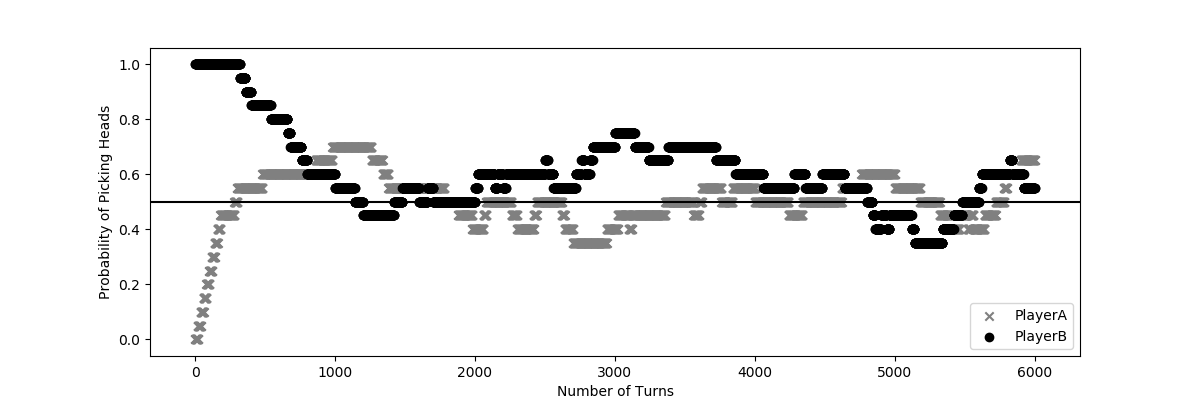
\includegraphics[scale=0.6]{../Figures/scatter_1.png}
\end{figure}

\FloatBarrier
\subsection{Rock-Paper-Scissors}

\subsubsection{Background}
In this game, two players each simultaneously reveal either rock, paper, or scissors. The players then  compare their choices and determine a winner with playoff +1 and a loser with playoff $-1$, a tie gives both players a payoff of 0. Rock beats scissors, scissors beats paper, paper beats rock, and all other combinations are a tie.

As in the matching-pennies game, rock-paper-scissors has no pure-strategy Nash equilibrium, but a mixed-strategy Nash equilibrium can be found by randomly picking rock, paper, or scissors with equal probability.


\subsubsection{Simulation}
A different method to show an equilibrium strategy is to map out all of the possible strategies and create distributions of both of their payoffs. If both players follow the same optimal strategy then the players should have the same payoff distribution. Since both players are the same, disregarding skill, and have access to the same choices and information, they should pick the mixed-strategy Nash equilibrium. 

Any payoff distributions that do not over lap can then be eliminated as possible optimal strategy. If one player is getting a lower payoff on average, then that player would adjust their strategy. This will continue until their payoffs converge. By simulating multiple mixed strategies and creating a distribution of each players payoffs the distributions that overlap should be the equilibrium.

From Figure 2, the players' payoffs converge at the mixed strategy Nash equilibrium weights. The top left graph is an example of when the weights favor player A, the top right favors player B, and the bottom graph is the equilibrium weights. As the weights get closer to equilibrium, the payoff distributions overlap.

\begin{figure}[h]
\caption{Histograms of Player Payoffs for Fixed-Weights}
\hspace*{-1.5cm} 
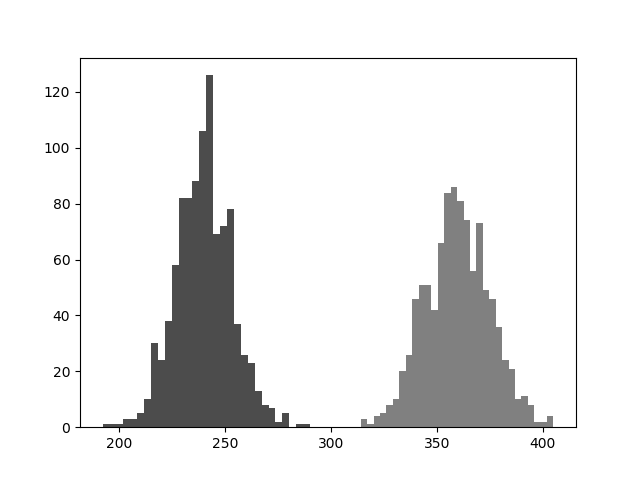
\includegraphics[width=0.6\textwidth]{../Figures/hist_1.png}%
\hfill
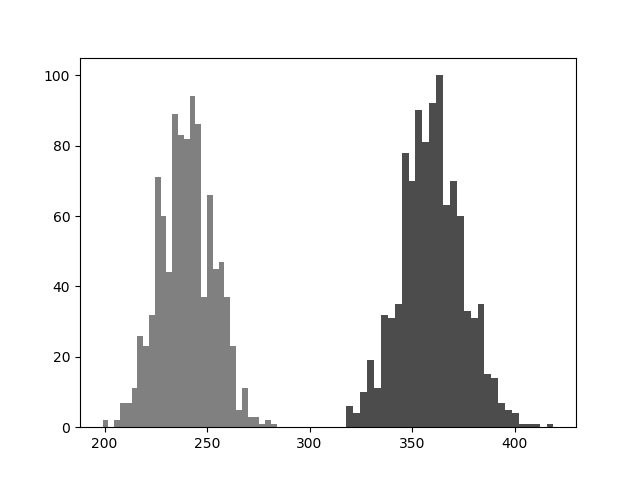
\includegraphics[width=0.6\textwidth]{../Figures/hist_3.png}%
\\
\hspace*{2.5cm} 
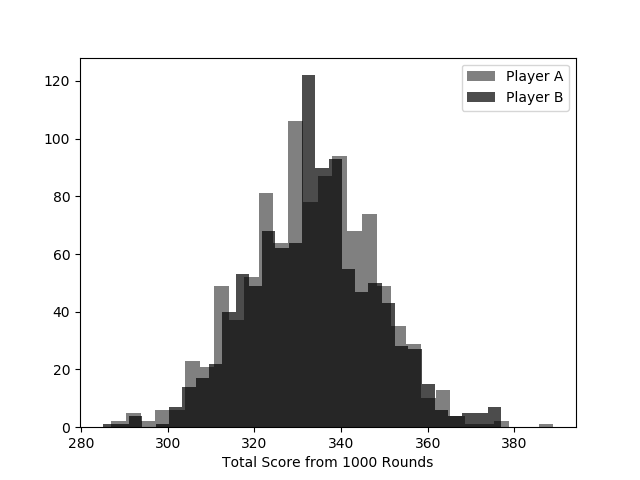
\includegraphics[width=0.6\textwidth]{../Figures/hist_2.png}
\end{figure}







\FloatBarrier
\section{Yu-Gi-Oh}
% Rules and simplified example game.

\subsection{Rules}
In a normal game of Yu-Gi-Oh, there are two players with separate forty card decks that they construct from the available card pool. At the beginning of the game, the players draw five cards from their decks, which are their hands. A player has a deck of cards; his hand---drawn from the deck; his field---cards played from the hand; and his graveyard---cards that were used and no longer in play. Players will decide who gets to go first through a random event---usually by rolling a die. At the start of the game each player has eight thousand life points. The main goal of the game is to reduce the opponent's life points to zero, thus winning the game, although a player can loose by running out of cards in their deck also known as decking out. Three main types of cards exist in the game: (1) monsters, (2) spells, and (3) traps. 

Monsters are used for attacking the opposing player's monsters and life points. Every monster has attack points---a whole number typically between zero and three thousand; in the simplified simulation all monsters will be the same with one thousand attack points. Monsters remain on the field unless destroyed by an opponent's monster or trap.

Spells are utility cards, they have a number of different abilities and uses, but for simplicity I shall limit them to one card. The chosen spell card can be used, from the hand or field, to destroy an opposing player's facedown spell or trap. During their turn, players can use their spells (from hand and field), keep them in hand, or set spells facedown on the field. Since the opposing player does not know if the card set on the field is a spell or trap it can be used to bluff the opponent into thinking it is a trap. Spells go to the graveyard immediately after use.  

Traps are disruption and defensive cards, they have a number of different abilities and uses, but for simplicity I shall limit them to one card. The chosen trap card can be used, from the field, to destroy an opposing player's attacking monster. Players can set traps on their turn, but can only use traps on the opposing player's turn. Traps, like spells, go to the graveyard immediately after use. 

In summary, monsters beat other monsters and damage an opposing player's life points; spells beat other spells or traps; and traps beat monsters.

Players take turns using the cards they have drawn. Each turn follows the order: Draw Phase, Main Phase 1, Battle Phase, Main Phase 2, and End Phase. I will be excluding the last two from my simulations for simplicity.

The draw phase is when the turn player draws a card from their deck, however, if a player has no cards left to draw they loose (decking out). 

Main phase 1 is when the turn player can use their spell cards from hand or field, place their spells or traps from hand to the field facedown, and summon (put on the field) monsters. Only the turn player can summon monsters and they can only summon a monster once during their turn. 

The battle phase is when the turn player uses their monsters to attack their opponent's monsters, except on the first turn. If the opponent has no monsters then the turn player can attack the opponent's life points instead by subtracting the monster's attack points from the player's life points, this is called attacking directly. When a monster attacks an opponent's monster the one with lower attack points is destroyed and placed in the graveyard. In the case of a tie, both monsters are destroyed. The difference in attack points is subtracted from the loosing player's life points. This is also when the opposing player can use their traps on field to destroy the turn player's attacking monsters.

After the turn ends, the cycle restarts with the next player and it continues until one or both of the players have lost all of their life points or decks out.

\subsection{Game Scenario}
For this example, the game will be simplified. Both players will have an infinitely sized deck with equal proportions of monsters, spells, and traps. They will start with no cards in hand, but still draw one card during their draw phase. The players will both only have 1 life point, so whoever successfully attacks directly wins.

Player A goes first, draws a card for turn and sets it facedown. 

Player B draws a monster for turn.

Now, what would player B want to do with this monster? Player B can choose to summon it or keep it for later and if player B summons it they can attack or leave it.

\subsection{Strategy}
Players should always choose to summon a monster if they can. While on the field monsters can defend their players' life points from opposing monsters and, as long as they do not attack, cannot be destroyed by traps. Since players can only summon one monster per their turn stock piling monsters in the hand is pointless, but having them on the field means more monsters to attack the opponents' life points with. Therefore, keeping it in hand should not happen.

To attack or to not attack? Since player B will summon their monster should they attack and risk loosing their only defense to a possible trap? If player B attacks one of two things can happen: player A's facedown is a trap and player B's monster is destroyed or the facedown is a spell and player B will win the game.

If player B attacks, then there is a fifty percent chance that the facedown card player A set is a trap and if it is, there is a one-third chance of player A drawing a monster and winning in the next turn. However, there is a fifty percent chance that the facedown is a bluff, a spell that cannot affect a monster, and player B can win by attacking directly for player A's last life point.

If player B does not attack, then player A will draw a card, take some action, and the cycle will continue until an attack is made. Since Player A has the advantage of going first, meaning that the player will always have one extra card on their turn, this cycle will favor the going first player.

In this simplified setting, the best response can be roughly solved for by comparing the expected values of each option. Outside of this setting, however, the game can be much too complex to solve normally. By simulating some of the possible outcomes of the game with different strategies and using a logistic regression model an approximation of the probability of winning can be made for each strategy. 

In this example, the strategy is a mixed-strategy of attack or do not attack. This decision is split into different groups based on what each player has on their field, for example, having a facedown versus just a monster. I shall go into more detail on the model later in this paper, but the results come from the formula below,
$$ \text{Pr(Player B wins)} = \frac{\exp(\beta_0 + \beta_1 x_1 + ... + \beta_K x_K)}{1 + \exp(\beta_0 + \beta_1 x_1 + ... + \beta_K x_K)}, \quad k=1,...K , $$
where $\beta_0, \beta_1, ..., \beta_K$ are the regression coefficients and $x_1,..., x_K$ are the mixed strategies. With the the strategy leaning towards attacking having the highest estimated probability of winning. Player B will want to risk the trap card to take advantage of player A's weakness before they can utilize their card advantage.






\section{Data}
% yugioh simulated data meaning and how it was made
\subsection{Yu-Gi-Oh Simulations}
The Yu-Gi-Oh games are simulated in Python by constructing rules, mentioned in the previous section, that the players must follow and marking points of interest as decision points. Decision points are binary moments in the game where a player can chose to take an action in a given circumstance or do nothing instead. One example would be if a player wants to attack when the opponent has a monster on their field and no spells or traps as well. The action would be to attack or not and the circumstances is the cards the opponent has.

The decision points are given weights, so players can pick with uneven probability. Each combination of weights for all of the decision points would be a possible strategy for a player to use. For instance, a player can choose the strategy of randomly picking with equal probability at each decision or another strategy is for a player to only take an action when the opponent has less monster. 

Taking into consideration all possible actions will make the state space too large and is computationally NP hard. Instead only a handful of decisions points are considered with the rest being concentrated out---given a fixed weight that the players cannot control. Certain decision points are fixed because, base on the rules of the game, deviating from them offers no possible reward. Consider a player deciding to summon a monster to his field. Monsters are the only way to win the game and can defend players from opposing player's monsters when necessary, so there are only advantages to having monsters on your field. Therefore, this decision was fixed so player always summon monsters if able.

The data collected from these simulations is the outcome of the game---win (1) or loose (0), binary variables representing whether a possible strategy---combination of weights---was used by each player or not, and which player went first.

Interestingly, the player who goes first is more likely to win, which is expected, however, as the game progresses the advantage that player has diminishes. In one setting, the game starts the players with no cards in hand and the players loose after taking damage once; this make the games shorter and the ``extra'' card the turn player gets by going first can make a bigger difference. For example, if the going first player draws monster cards twice in a row at the beginning, then they win no matter what the other player does. When players start with more cards in hand and have more life points the advantage of going first should shrink.







\section{Approximate the Optimal Solution}
% logistic regression and adjustment function

\subsection{Adjustment Function}

From a model including player actions at decision points, finding which actions positively affect a player and by how much can be estimated, see \cite{Shanahan:1984}.

The coefficients from a logistic regression are the log of the odd ratios for the variables.
$$ \text{Logit[Pr(Y=1)] = log(odds)} $$
$$ \exp[\text{log(odds)] = odds} $$
$$ \text{Pr(Y} = 1) = \frac{\text{odds}}{1+\text{odds}} $$
\begin{equation}
 \text{Pr(Y = 1)} = \frac{\exp(\beta_0 + \beta_1 x_1 + ... + \beta_K x_K)}{1 + \exp(\beta_0 + \beta_1 x_1 + ... + \beta_K x_K)}, \quad k=1,...K , 
 \end{equation}
where Y is the binary outcome variable for win(1) or loose(0); $\beta_0, \beta_1, ..., \beta_K$ are the regression coefficients; and $x_1,..., x_K$ are the mixed strategies.

% talk about the basket ball paper
% talk about dynamic programming 
% roulette

In 1961, Edward Thorp and Claude Shannon made a wearable computer that could estimate which five-slot section a ball would landed in when placed in a spinning roulette wheel, see \cite{Thorp:2017}. The idea was that they could input the current state of the spinning roulette---speed, tilt of the board, etc.---and then estimate where the ball would land from a predetermined reference point. Similarly, the adjustment function can be used to predict what the optimal strategy is in a current state. By inputing the cards that are currently in play and then simulating a thousand games with varying strategies, a logistic regression can used to predict who would win in that current state. The coefficients from this regression can be inputed into Equation (1) and evaluated at varying mixed strategies to find which combination of weights maximizes the probability of winning.






\section{Conclusions}
% compare the different strategies payoffs 
% predict winner based on which strategy each player employed

\subsection{Adjustment Model}
At first, the adjustment function would reevaluate itself in every new state the player encountered, every turn the state space would be updated and new coefficients would be estimated to solve for new weights. This, however, turned out to be too computationally expensive and thus, to minimize complexity, a separate set of simulated games were used to approximate a model that utilizes a few initial state variables to estimate the coefficients. 

The estimated model $Pr(Y=1 | X = x) = \log \frac{p}{1-p} = \beta_0 + \beta_1 x_1 + ... + \beta_K x_K, \quad k = 1,...,K$, see table 1 for results, used FirstA---a binary variable for player A going first; HAMon, HASpell, HATrap---the number of monsters, spells, and traps in the players hand receptively; and PrAW---the weights for the decision player A has to make. 

The decision points are when a player wants to attack with his monsters in different scenarios and the weights are the probability that he takes that action. PrAwMST is attacking when the opponent has monster and spells or traps; PrAwM is attacking when the opponent has only monsters; and PrAwST is attacking when the opponent only has spells or traps. The coefficients on the weights decrease as the risk of loosing a monster increases; the decision with the greatest risk is PrAMST followed by PrAwM and PrAST. A player can lose a monster from an opposing monster and a potential trap at PrAMST, so PrAST is the safest since spells cannot hurt monsters.

Interestingly, players were better off when they drew more spells and traps rather than monsters. Originally, I assumed monsters would be the most important card, given that they are the only way to win the game outside of decking the opponent out (runs out of cards to draw thus losing). After seeing the regression and reconsidering the rules of the game, I speculate this occurred due to monsters only being allowed to be summoned once per turn. Similar to pouring too much water into a funnel, at some point it will overflow if you pour more than the funnel can let out. A player can safely win a game with only one monster provided his opponent is more aggressive---attacking into traps. 

{\footnotesize
\begin{table}
\caption{Logistic Model: Starting State}
\begin{center}
\begin{tabular}{lc}
\hline
          & Dependent Variable:   \\
          &  win (1) or lose (0)  \\
\midrule
Intercept & 0.115                 \\
          & (0.127)               \\
FirstA    & 1.132***              \\
          & (0.081)               \\
HAMon     & -0.284***             \\
          & (0.017)               \\
HASpell   & 0.158***              \\
          & (0.028)               \\
HATrap    & 0.806***              \\
          & (0.030)               \\
PrAwMST   & -0.679***             \\
          & (0.064)               \\
PrAwM     & -0.177***             \\
          & (0.064)               \\
PrAwST    & -0.090                \\
          & (0.064)               \\
N         & 27440                 \\
\hline
\end{tabular}
\end{center}
\end{table}
}

\FloatBarrier
\subsection{Strategy Evaluation}
In this model after simulating each game, the strategy player A employed would be recorded as a binary variable: AsHalf---random play, player A effectively flipped a coin to decide his actions; AsAlways---always take an action if possible; and AsADP---the weights were estimated from the coefficients from table 1 and cards in their hand. Player B's strategy is randomly assigned between random play and always play in order to represent player A's lack of knowledge of player B's strategy. The strategies can be thought of as how aggressive the player wants to be, always attacking as opposed to the more passive attacking half of the time. The AsADP was somewhat of a middle ground between the two, since it changed based on the player's hand.

Initial inspection confirmed that going first is advantageous since it is always the largest positive coefficient. This showed in the simulations as well, the player going first usually won two-thirds of the time. An unusual result was that the random play strategy did so well in comparison to the others. Saving the monsters to keep as a wall while passively applying pressure is about as good as a player a do unless he can tell when the opponent is bluffing (setting a spell but behaving like it is a trap). I had wanted to further study more passive strategies, however, this leads to long games that end in decking out and increasing the simulation time. Regardless a passive strategy would force the first turn player to act more aggressively, since if the players have the same deck size, then the player going first will run out of cards first.

As with matching-pennies, if both players are employing the same strategy, optimal or otherwise, with the same deck then each player should expect to win approximately half of the games played. 


{\footnotesize
\begin{table}
\caption{Logistic Model: Evaluate Strategies}
\begin{center}
\begin{tabular}{lc}
\hline
          & Dependent Variable:   \\
          &  win (1) or lose (0)  \\
\midrule
Intercept & -0.973***             \\
          & (0.082)               \\
FirstA    & 2.691***              \\
          & (0.160)               \\
AsHalf    & -0.334***             \\
          & (0.117)               \\
AsAlways  & -0.397***             \\
          & (0.116)               \\
AsADP     & -0.242**              \\
          & (0.115)               \\
N         & 960                   \\
\hline
\end{tabular}
\end{center}
\end{table}
}







\FloatBarrier
\section*{Appendix}
\appendix

\section{Matching Pennies}

\lstinputlisting[language=python]{../MatchingPennies/original_MP.py}

The matching pennies script is meant to show how players can evolve over time and can converge to an optimal solution. The first two functions are the players and their strategy is how much weight they give to the choices (heads or tails). The next function adjusts the loosing player's strategy by increments of 0.05 based on the history of the last 20 outcomes. The game function keeps track of the score and calls the weight adjusting function every 20 turns. After about 1000 simulations it settles down, with some error, to about 0.5.

\FloatBarrier
\begin{table}[]
\caption{Matching Pennies (First 10 Simulations)}
\begin{tabular}{lllllll}
\hline
A & B & ScoreA & ScoreB & Turns & WeightA\_heads & WeightB\_heads \\
\hline
T & H & 0.0    & 1.0    & 1.0   & 0.0            & 1.0            \\
T & H & 0.0    & 2.0    & 2.0   & 0.0            & 1.0            \\
T & H & 0.0    & 3.0    & 3.0   & 0.0            & 1.0            \\
T & H & 0.0    & 4.0    & 4.0   & 0.0            & 1.0            \\
T & H & 0.0    & 5.0    & 5.0   & 0.0            & 1.0            \\
T & H & 0.0    & 6.0    & 6.0   & 0.0            & 1.0            \\
T & H & 0.0    & 7.0    & 7.0   & 0.0            & 1.0            \\
T & H & 0.0    & 8.0    & 8.0   & 0.0            & 1.0            \\
T & H & 0.0    & 9.0    & 9.0   & 0.0            & 1.0            \\
T & H & 0.0    & 10.0   & 10.0  & 0.0            & 1.0           \\
\hline
\end{tabular}
\end{table}


\FloatBarrier
\section{Rock-Paper-Scissors}

\begin{lstlisting}
import random
import pandas as pd

def PlayerA(weightA, n):
    Player_A = random.choices(population=['Rock','Paper', 'Scissors'],weights=weightA, k=n)
    return Player_A
    
def PlayerB(weightB, n):
    Player_B = random.choices(population=['Rock','Paper', 'Scissors'],weights=weightB, k=n)
    return Player_B

def Game(x, wA, wB):
    scoreA = 0
    scoreB = 0
    turns = x
    history = pd.DataFrame() 
    A = PlayerA(wA, x)
    B = PlayerB(wB, x)
    
    for play in range(x):
        if A[play] == B[play]:
            pass
        elif A[play] == 'Rock':
            if B[play] == 'Paper':
                scoreB += 1
            else:
                scoreA += 1    
        elif A[play] == 'Paper':
            if B[play] == 'Scissors':
                scoreB += 1
            else:
                scoreA += 1
        else:
            if B[play] == 'Rock':
                scoreB += 1
            else:
                scoreA += 1
            
    history = history.append({'Turns':turns, 'ScoreA':scoreA, 'ScoreB':scoreB,
                              'wA_Rock':wA[0], 'wA_Paper':wA[1], 'wA_Scissors':wA[2],
                              'wB_Rock':wB[0], 'wB_Paper':wB[1], 'wB_Scissors':wB[2],
                              'weights_A':str(wA), 'weights_B':str(wB)}, ignore_index=True)
                    
    return history

fixed = pd.DataFrame()
for play in range(0,1000):
    fixed = fixed.append(Game(1000, [0.2, 0.6, 0.2], [0.4, 0.5, 0.1]))
\end{lstlisting}

The rock-paper-scissors script plays out multiple games at fixed strategies and then I can compare the distributions of the players payoffs to look for a combination of strategies where the payoffs overlap. The first two functions are the players and their strategy is how much weight they give to the choices (rock, paper, or scissors). It is slightly different from matching pennies because instead of a single game the functions are set to pick a vector of n games at a time. The game function then keeps track of the score for each n game and records the total. I run a thousand of these vector games at a time for a fixed weight and create a distribution of each player's score. 

\FloatBarrier
\begin{table}[]
\caption{Rock-Paper-Scissors (First 10 Simulations)}
\begin{tabular}{lllll}
\hline
ScoreA & ScoreB & Turns  & weights\_A          & weights\_B          \\
\hline
335.0  & 252.0  & 1000.0 & {[}0.2, 0.6, 0.2{]} & {[}0.4, 0.5, 0.1{]} \\
363.0  & 232.0  & 1000.0 & {[}0.2, 0.6, 0.2{]} & {[}0.4, 0.5, 0.1{]} \\
394.0  & 223.0  & 1000.0 & {[}0.2, 0.6, 0.2{]} & {[}0.4, 0.5, 0.1{]} \\
344.0  & 255.0  & 1000.0 & {[}0.2, 0.6, 0.2{]} & {[}0.4, 0.5, 0.1{]} \\
358.0  & 242.0  & 1000.0 & {[}0.2, 0.6, 0.2{]} & {[}0.4, 0.5, 0.1{]} \\
363.0  & 253.0  & 1000.0 & {[}0.2, 0.6, 0.2{]} & {[}0.4, 0.5, 0.1{]} \\
356.0  & 233.0  & 1000.0 & {[}0.2, 0.6, 0.2{]} & {[}0.4, 0.5, 0.1{]} \\
367.0  & 229.0  & 1000.0 & {[}0.2, 0.6, 0.2{]} & {[}0.4, 0.5, 0.1{]} \\
362.0  & 232.0  & 1000.0 & {[}0.2, 0.6, 0.2{]} & {[}0.4, 0.5, 0.1{]} \\
365.0  & 232.0  & 1000.0 & {[}0.2, 0.6, 0.2{]} & {[}0.4, 0.5, 0.1{]} \\
\hline
\end{tabular}
\end{table}

\FloatBarrier
\section{Yu-Gi-Oh}

\lstinputlisting[language=python]{../Game/rules_hand_field.py}
\lstinputlisting[language=python]{../Game/mechanics_cs.py}
\lstinputlisting[language=python]{../Game/turns_4.py}
\lstinputlisting[language=python]{../Game/max_weightFunc_2.py}
\lstinputlisting[language=python]{../Game/currnent_state.py}


The Yu-Gi-Oh scripts plays a single game at a time and outputs the strategy used along with the weights for each decision point. In table 5, the columns are FirstA---if player A went first; HA---how many of each card type was in player A's hand; LP\_A---if player A won or not; PrAw---the weights for each decision point; and As/Bs---if a strategy was used by a player. 

The scripts follow the rules as highlighted in section 3 and the script will loop until a win condition is met. The script is broken up into general rules, phases of a turn, and a full turn for both players.


\FloatBarrier
{\footnotesize
\begin{table}[]
\caption{Yu-Gi-Oh cards in hand and attack weights}
\begin{tabular}{rrrrrrrr}
\toprule
 FirstA &  HAMon &  HASpell &  HATrap &  LP\_A &  PrAwM &  PrAwMST &  PrAwST \\
\midrule
    0.0 &    2.0 &      2.0 &     1.0 &   0.0 &    1.0 &      1.0 &     1.0 \\
    1.0 &    2.0 &      0.0 &     0.0 &   1.0 &    1.0 &      1.0 &     1.0 \\
    1.0 &    2.0 &      0.0 &     0.0 &   0.0 &    1.0 &      1.0 &     1.0 \\
    0.0 &    2.0 &      0.0 &     3.0 &   1.0 &    1.0 &      1.0 &     1.0 \\
    0.0 &    2.0 &      1.0 &     2.0 &   0.0 &    1.0 &      1.0 &     1.0 \\
    0.0 &    1.0 &      1.0 &     3.0 &   0.0 &    1.0 &      1.0 &     1.0 \\
    1.0 &    1.0 &      0.0 &     0.0 &   1.0 &    1.0 &      1.0 &     1.0 \\
    1.0 &    3.0 &      0.0 &     0.0 &   1.0 &    1.0 &      1.0 &     1.0 \\
    1.0 &    2.0 &      0.0 &     0.0 &   0.0 &    1.0 &      1.0 &     1.0 \\
    0.0 &    3.0 &      1.0 &     1.0 &   1.0 &    1.0 &      1.0 &     1.0 \\
\bottomrule
\end{tabular}

\end{table}
}
{
\begin{table}[]
\caption{Yu-Gi-Oh strategy used and attack weights}
\scriptsize
\begin{tabular}{rrrrrrrrrrr}
\toprule
 AsADP &  AsAlways &  AsHalf &  BsAlways &  BsHalf &  FirstA &  LP\_A &  LP\_B &  PrAwM &  PrAwMST &  PrAwST \\
\midrule
   0.0 &       1.0 &     0.0 &       1.0 &     0.0 &     0.0 &   0.0 &   1.0 &    1.0 &      1.0 &     1.0 \\
   0.0 &       1.0 &     0.0 &       1.0 &     0.0 &     0.0 &   0.0 &   1.0 &    1.0 &      1.0 &     1.0 \\
   0.0 &       1.0 &     0.0 &       1.0 &     0.0 &     1.0 &   1.0 &   0.0 &    1.0 &      1.0 &     1.0 \\
   0.0 &       1.0 &     0.0 &       1.0 &     0.0 &     1.0 &   1.0 &   0.0 &    1.0 &      1.0 &     1.0 \\
   0.0 &       1.0 &     0.0 &       1.0 &     0.0 &     1.0 &   1.0 &   0.0 &    1.0 &      1.0 &     1.0 \\
   0.0 &       1.0 &     0.0 &       1.0 &     0.0 &     0.0 &   0.0 &   1.0 &    1.0 &      1.0 &     1.0 \\
   0.0 &       1.0 &     0.0 &       1.0 &     0.0 &     1.0 &   1.0 &   0.0 &    1.0 &      1.0 &     1.0 \\
   0.0 &       1.0 &     0.0 &       1.0 &     0.0 &     0.0 &   0.0 &   1.0 &    1.0 &      1.0 &     1.0 \\
   0.0 &       1.0 &     0.0 &       1.0 &     0.0 &     1.0 &   1.0 &   0.0 &    1.0 &      1.0 &     1.0 \\
   0.0 &       1.0 &     0.0 &       1.0 &     0.0 &     0.0 &   0.0 &   1.0 &    1.0 &      1.0 &     1.0 \\
\bottomrule
\end{tabular}

\end{table}
}





\FloatBarrier
\nocite{*}
\bibliographystyle{chicago}
\bibliography{References}


\end{document}



